% Anforderungen  an  Stabilität,  Robustheit,  Leistungsfähigkeit  etc.  des Systems.  Dies  beinhaltet  auch  den  Umgang  mit  fehlerhaften  Eingabedaten  oder  fehlerhaften Konfigurationen.
Durch begrenzte zeitliche und widersprüchliche Anforderungen der Qualitätsziele können nicht alle Qualitätsziele vollständig erfüllt werden.
Im Folgenden Kapitel wird die Priorisierung der Qualitätsziele vorgestellt.
Die Hauptqualitätsmerkmale sind Funktionalität, Zuverlässigkeit, Benutzbarkeit, Effizienz, Änderbarkeit und Übertragbarkeit.
\section{Übersicht}
Es folgt eine detaillierte Tabelle der Gewichtung aller Qualitätsziele.
Zur Erläuterung dieser werden alle Qualitätsziele und deren Bedeutungen im Kontext des Programmes vorgestellt.
\begin{normalsize}

\end{normalsize}
\subsubsection{Funktionalität}
\begin{itemize}
\item Richtigkeit - Korrektheit der Zwischen und Endergebnisse bei korrekten Algorithmen
\item Interoperabilität - Direkte Zusammenarbeit des Programms mit anderen Programmen
\item Ordnungsgenmäßigkeit - Plangemäße Ausführung der Funktionen ohne Fehler 
\item Sicherheit - Kryptische Sicherheit des Programms 
\end{itemize}
\subsubsection{Zuverlässigkeit}
\begin{itemize}
\item Reife - Bugfreiheit der Software
\item Fehlertoleranz - Zuverlässigkeit bei Fehlern in Plugins
\item Robustheit - Zuverlässigkeit bei falschen Benutzereingaben und Daten
\item Wiederherstellbarkeit - Wiederherstellung des Programms nach starken Fehlern
\end{itemize}
\subsubsection{Benutzbarkeit}
\begin{itemize}
\item Verständlichkeit - Verständnis und Anschaulichkeit für Erstbenutzer
\item Erlernbarkeit - Geringer zeitlicher Aufwand zur Einarbeitung
\item Bedienbarkeit - Anzahl an Interaktionen um eine gewünschte Funktion durchzuführen
\end{itemize}
\newpage
\subsubsection{Effizienz}
\begin{itemize}
\item Zeitverhalten - Zeitdauer um Funktionen auszuführen (maßgeblich von Algorithmenplugins abhängig)
\item Verbrauchsverhalten - Ressourcenverbrauch um Funktionen auszuführen (maßgeblich von Algorithmenplugins abhängig)
\end{itemize}
\subsubsection{Änderbarkeit} 
Änderbarkeit wird im Kontext zum 3dMuVi-Programm hauptsächlich auf die Pluginstruktur bezogen.
\begin{itemize}
\item Analysierbarkeit - Verständlichkeit und Dokumentation der Plugin-Schnittstellen
\item Modifizierbarkeit - Modfizierbarkeit mit Hilfe von Plugins zu den gebotenen Schnittstellen
\item Stabilität - Stabilität nach Anpassungen mittels funktionstüchtigen Plugins 
\item Prüfbarkeit - Testbarkeit nach Anpassungen mittels funktionstüchtigen Plugins 
\end{itemize}
\subsubsection{Übertragbarkeit}
\begin{itemize}
\item Installierbarkeit - Installieraufwand für Systeme, die Hardware- und Softwareanforderungen erfüllen
\item Anpassbarkeit - Mögliche spätere Anpassung auf andere Systeme   
\item Austauschbarkeit - Austauschbarkeit der Software durch andere Software 
\end{itemize}

\begin{normalsize}

\end{normalsize}
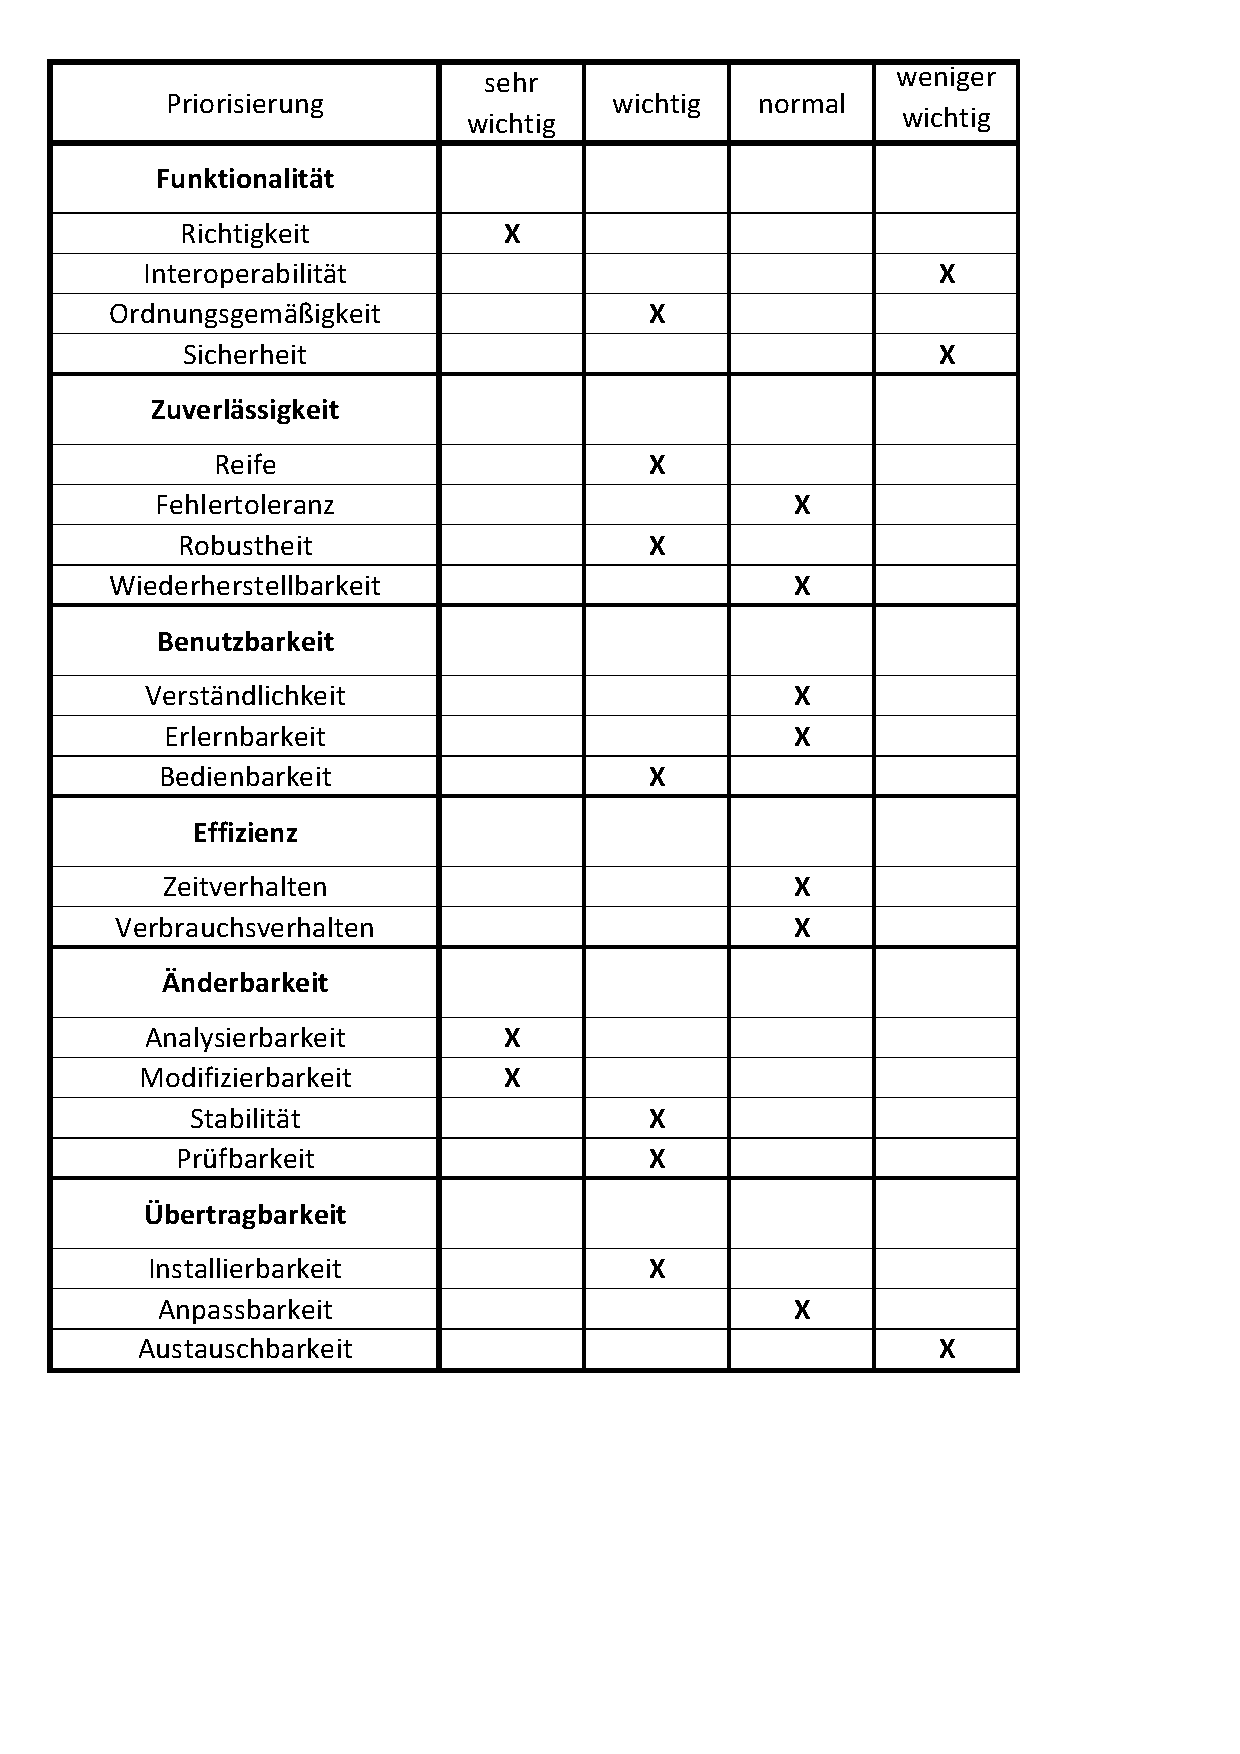
\includegraphics[width=1.15\textwidth]{img/Quali.pdf}
\begin{normalsize}

\end{normalsize}

\section{Zusammenfassung}
 
\begin{itemize}
\item Der Hautfokus der Software liegt auf korrekter Funktionsweise und Erweiterungen mit Hilfe von Plugins (Hauptsächlich weitere Algorithmen und Workflows).  
\item wichtige Qualitätsmerkmale sind gute Bedienbarkeit bei fachlichem Verständnis und Zuverlässigkeit, solange funktionstüchtige Algorithmen verwendet werden. Außerdem soll das Programm ohne großen Aufwand auf einem Linux-System installierbar sein.
\item Die Effizienz des Programms ist kaum beeinflussbar, da sie hauptsächlich von den verwendeten Algorithmen und Parametern dieser abhängt.
\item Sicherheit, Interoperabilität und Austauschbarkeit werden als weniger wichtig erachtet, da das Programm eigenständig und auf einzelnen Computern ausgeführt wird.
\end{itemize}